\documentclass[11pt]{article}
\usepackage{amsmath, amssymb, graphicx, hyperref}
\usepackage[a4paper,margin=1in]{geometry}

\title{Analysis of Four Particles in a Periodic Cosine Potential}
\author{}
\date{}

\begin{document}

\maketitle

\section{Introduction}

In this study, we analyze the behavior of four quantum particles in a one-dimensional periodic potential defined by a cosine function. The primary focus is to investigate the effects of spin configurations and spatial arrangements on the energy of the system. Specific scenarios include cases where the particles are either spatially separated, two of them are neighbors with opposite spins, two neighbors with the same spin, or three neighbors with the same spin.

The analysis is conducted in the absence of direct electron-electron interactions (e.g., no Coulomb repulsion), with the energy contributions arising purely from the kinetic energy and the influence of the external potential. The mathematical formulation and detailed results are presented below.

\section{Mathematical Framework}

\subsection{Potential and Wavefunctions}

The periodic potential is defined as:
\begin{equation}
V(x) = -A \cdot \cos(2 \pi a x),
\end{equation}
where \(\text{AmpPot}\) is the amplitude of the potential, and \(a\) is the periodicity parameter.

Each particle's spatial wavefunction is constructed as a localized Gaussian indexed by \(i\), where \(i\) counts the basis functions and each basis function is centered at a specific potential minimum \(\tilde{x}_{i}\) and has a specific spin \(\tilde{\sigma}_i\), and has a width parameter \(\alpha_i\):
\begin{equation}
\phi_\text{spatial}(x, i) =  \cdot e^{-\alpha_i \cdot (x - \tilde{x}_{i})^2},
\end{equation}
where \(\alpha_\text{center}\) determines the localization width of the particle's wavefunction.

The spin wavefunction is represented as a Kronecker delta function:
\begin{equation}
\chi_{spin}(\sigma, \tilde{\sigma}) = \delta_{\sigma, \tilde{\sigma}}.
\end{equation}

The total wavefunction for each particle is the product of its spatial and spin parts:
\begin{equation}
\phi(x, \sigma, \text{i}, \tilde{\sigma}) = \phi_\text{spatial}(x, \text{i}) \cdot \chi_\text{spin}(\sigma, \tilde{\sigma}).
\end{equation}

\subsection{Total Wavefunction}

The total wavefunction for the four particles is constructed as a Slater determinant to satisfy fermionic antisymmetry:
\begin{equation}
\Psi_\text{total}(\vec{x}, \vec{\sigma}) = \sum_{\tilde{\sigma}} \text{Det}
\begin{bmatrix}
\phi(x_1, \sigma_1, 1, \tilde{\sigma}_1) & \cdots & \phi(x_1, \sigma_1, 4, \tilde{\sigma}_4) \\
\vdots & \ddots & \vdots \\
\phi(x_4, \sigma_4, 1, \tilde{\sigma}_1) & \cdots & \phi(x_4, \sigma_4, 4, \tilde{\sigma}_4)
\end{bmatrix},
\end{equation}
where the summation is over all valid spin configurations.

\subsection{Energy Calculation}

The total energy is the expectation value of the Hamiltonian, incorporating kinetic and potential energy terms:
\begin{equation}
E = \int \Psi_\text{total}^*(\vec{x}, \vec{\sigma}) \left[ -\frac{1}{2} \sum_{i=1}^4 \nabla_i^2 + \sum_{i=1}^4 V(x_i) \right] \Psi_\text{total}(\vec{x}, \vec{\sigma}) \; dx_1 \cdots dx_4.
\end{equation}

The integrals are evaluated analytically for various configurations to determine the total energy in each case. The total energy is minimized with respect to the localization width parameters \(\alpha_i\).

\section{Results}

We consider the following scenarios:

\subsection{All Four Particles Separated}
In this configuration, each particle is localized in a separate well. The total energy per particle is calculated to be:
\begin{equation}
E_\text{separated} = -0.0323 \, \text{per particle}.
\end{equation}

\begin{figure}[h]
    \centering
    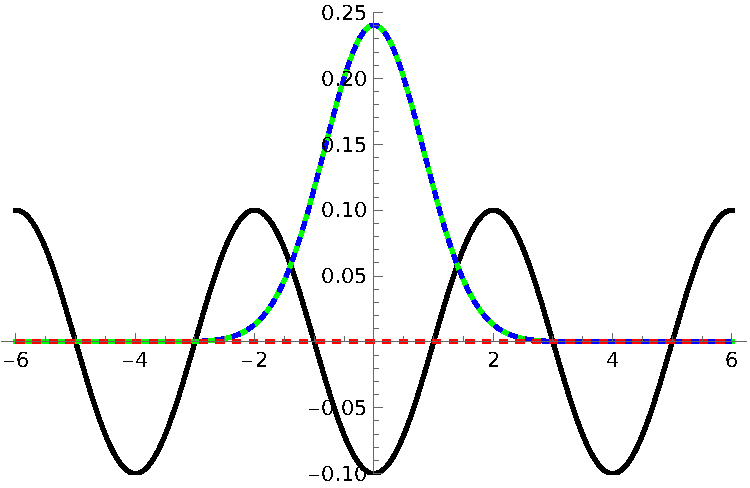
\includegraphics[width=0.8\textwidth]{IMGseparated.pdf}
    \caption{Potential and density for all particles separated.}
    \label{fig:separated}
\end{figure}

\subsection{Two Neighboring Particles with Opposite Spins}
When two particles with opposite spins are placed in neighboring wells, their spatial wavefunctions can overlap due to the symmetric spatial configuration. However, this overlap does not result in a significant energy change due to the absence of electron-electron interactions. The energy per particle is:
\begin{equation}
E_\text{opposite\_spin\_neighbor} = -0.0323 \, \text{per particle}.
\end{equation}

\begin{figure}[h]
    \centering
    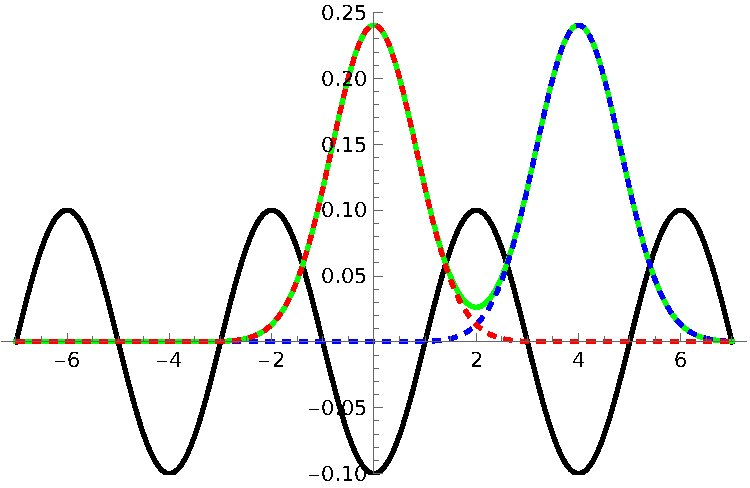
\includegraphics[width=0.8\textwidth]{IMGopposite_spin_neighbor.pdf}
    \caption{Potential and density for two neighboring particles with opposite spins.}
    \label{fig:opposite_spin_neighbor}
\end{figure}

\subsection{Two Neighboring Particles with Same Spins}
For two particles with the same spin in neighboring wells, the antisymmetric nature of the spatial wavefunction suppresses overlap, resulting in no significant energy difference compared to configurations where the particles are farther apart. The energy per particle remains:
\begin{equation}
E_\text{same\_spin\_neighbor} = -0.0305 \, \text{per particle}.
\end{equation}

\begin{figure}[h]
    \centering
    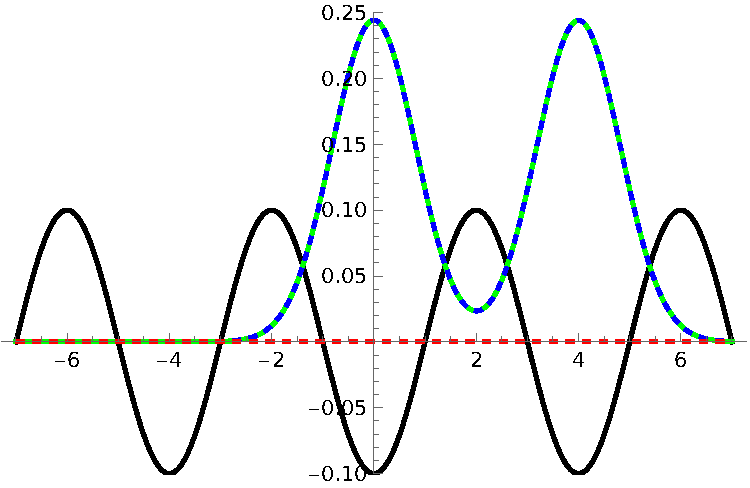
\includegraphics[width=0.8\textwidth]{IMGsame_spin_neighbor.pdf}
    \caption{Potential and density for two neighboring particles with same spins.}
    \label{fig:same_spin_neighbor}
\end{figure}

\subsection{Three Neighboring Particles with Same Spins}
When three particles with the same spin are placed in neighboring wells, the antisymmetric spatial wavefunction continues to suppress overlap. This configuration also results in no significant energy change due to the lack of inter-particle interactions. The energy per particle is:
\begin{equation}
E_\text{three\_same\_spin} = -0.0299 \, \text{per particle}.
\end{equation}

\begin{figure}[h]
    \centering
    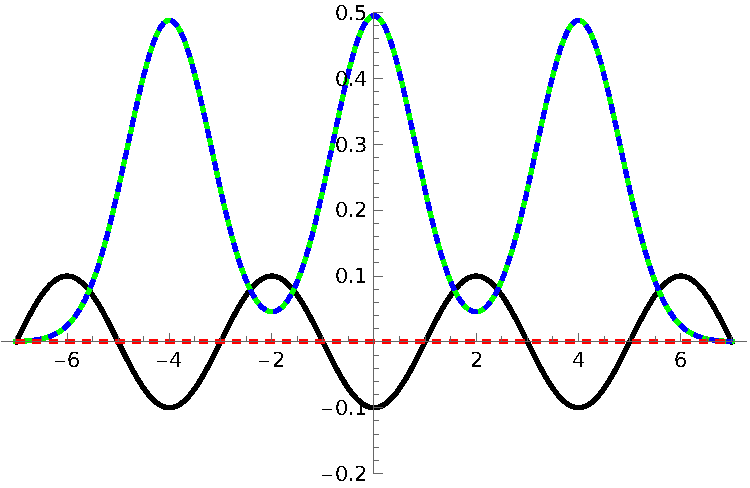
\includegraphics[width=0.8\textwidth]{IMGthree_same_spin.pdf}
    \caption{Potential and density for three neighboring particles with same spins.}
    \label{fig:three_same_spin}
\end{figure}

\section{Conclusion}

From the calculations, we observe:
\begin{itemize}
    \item For particles with the same spin an increase of the total energy is observed, which can be interpreted as "exchange energy", as no other interactions (e.g. electron-electron interaction) are present.
    \item For particles with opposite spins no change of the total energy is observed, therefore it is difficult talk about "exchange interaction" in this case.
\end{itemize}

With this in mind we will further investigate more complex situations, for example j-T models. "This document was prepared with the assistance of AI tools."
\end{document}
